% CHAPTER 3

\chapter{ROS}\label{ch:ros}
\ac{ROS} \cite{ROS} nasce nel 2007 sotto il nome di Switchyard presso lo Stanford Artificial Intelligence Laboratory (SAIL), centro di eccellenza per la ricerca sull'intelligenza artificiale della Stanford University, in California. Nello specifico, viene sviluppato inizialmente da due dottorandi dell'università a capo del programma Personal Robotics (PR) per fornire supporto al progetto Stanford Artificial Robot (STAIR). Nel 2008 lo sviluppo del progetto progredisce presso il Willow Garage (diventando \acs{ROS}), ente di ricerca e incubatore nel campo della robotica, che versa il proprio contributo approfondendo i principi con cui il progetto nasce e realizzando le prime versioni testate.\\

Brevemente, si tratta di un middleware open source basato su sistemi operativi Linux (e.g. Ubuntu) che consente comunicazione tra processi attraverso un meccanismo basato sul passaggio di messaggi. Praticamente, comprende un insieme di librerie, strumenti e convenzioni che semplificano lo sviluppo di software impiegato nei robot.\\

\acs{ROS} non è stato inizialmente progettato e rilasciato per un uso di tipo industriale, ma con l'obiettivo di velocizzare la ricerca sulla robotica. Per questo motivo, alcuni aspetti come la sicurezza oppure il supporto per programmi real-time non sono stati considerati essenziali. L'espansione di \acs{ROS} in ambito industriale ha dato vita alla creazione di \acs{ROS} 2 \cite{ROS2}: una riprogettazione completa del framework che mantiene le funzioni principali e risolve le carenze riscontrate nella prima versione.

% ------------------------------ FS LEVEL ------------------------------

\section{Filesystem Level}
Il \emph{Filesystem Level} è l'organizzazione del framework all'interno della macchina. Comprende tutte le risorse utilizzate: \emph{packages}, \emph{metapackages}, \emph{package manifests}, \emph{repositories}, \emph{message types}, \emph{service types}.

\subsection{Packages}
I \emph{packages} sono l'unità di organizzazione del software a questo livello in \acs{ROS}. Contengono file di configurazione e file eseguibili (\emph{nodes}, trattati nel seguito) e contribuiscono, insieme alle \emph{repositories}, alla modularità del framework. Infatti, si cerca di creare e mantenere \emph{packages} di dimensioni contenute e semplici da utilizzare.

% ------------------------------ CG LEVEL ------------------------------

\section{Computation Graph Level}
Il \emph{Computation Graph Level} è dove viene processata ed elaborata l'informazione. Si tratta di una rete peer-to-peer costituita da tutti i processi attivi in \acs{ROS} che stanno processando ed elaborando dati insieme.

\subsection{Nodes}
Un \emph{node} è un processo che compie una qualsiasi attività computazionale all’interno del sistema \acs{ROS}.\\

Essendo \acs{ROS} progettato per essere modulare, tipicamente un sistema basato su di esso comprende numerosi nodi e in tal contesto sono interpretabili come moduli software, ognuno dei quali è incaricato di gestire un aspetto del comportamento del robot (e.g. parte decisionale, movimento, azionamento motori, ecc.).\\

Un sistema il cui carico computazionale venga ripartito tra i vari nodi di cui è costituito ha innanzitutto il vantaggio di una maggiore tolleranza agli errori, potendo gestire indipendentemente il malfunzionamento del singolo nodo. La complessità del codice è ridotta se confrontata coi sistemi monolitici e i dettagli implementativi sono nascosti in quanto i singoli nodi offrono un’interfaccia composta da una \ac{API} minimale.\\

Ogni nodo in esecuzione dispone di un cosiddetto "graph resource name", cioè un nome che lo identifica unicamente nel sistema, e di un tipo, che semplifica il processo di indirizzamento nel filesystem.

\subsection{Master}
In un sistema basato su ROS, il \emph{master} è un server centralizzato che offre ai nodi un servizio di registrazione e di naming, similmente all’informazione data da un server \ac{DNS}. Permette infatti al singolo nodo di contattarne un secondo attraverso una metodologia peer-to-peer. Tiene inoltre traccia per ogni singolo \emph{topic} (trattati nel seguito) dei relativi nodi publisher e subscriber. Il \emph{master} offre anche il parameter server, cioè un server che offre un servizio di memorizzazione e consultazione di parametri a tempo di esecuzione (runtime) ai nodi che ne richiedono i servizi attraverso una \acs{API} di rete.
 
\subsection{Topics}
I \emph{topic} costituiscono il mezzo di comunicazione asincrono, unidirezionale, per lo scambio di messaggi tra nodi, secondo una semantica di tipo publish/subscribe (pubblica/sottoscrivi). Ci possono essere più nodi publisher e subscriber concorrenti per un singolo \emph{topic} e un singolo nodo può pubblicare e/o sottoscriversi a più \emph{topics}. In generale, i nodi publisher e subscriber non sono consapevoli dell’esistenza degli altri, disaccoppiando così la produzione dell’informazione dal suo consumo.\\

Ogni \emph{topic} è fortemente tipizzato dal tipo di messaggio che viene pubblicato e i nodi possono ricevere esclusivamente messaggi il cui tipo sia compatibile. Ciò determina che all’interno del \emph{topic} sia possibile scrivere o leggere un solo tipo di messaggio.\\

Il protocollo di trasporto utilizzato per lo scambio dei messaggi viene definito in fase di esecuzione e può essere di due tipi: TCPROS o UDPROS.

\begin{figure}[H]
    \centering
    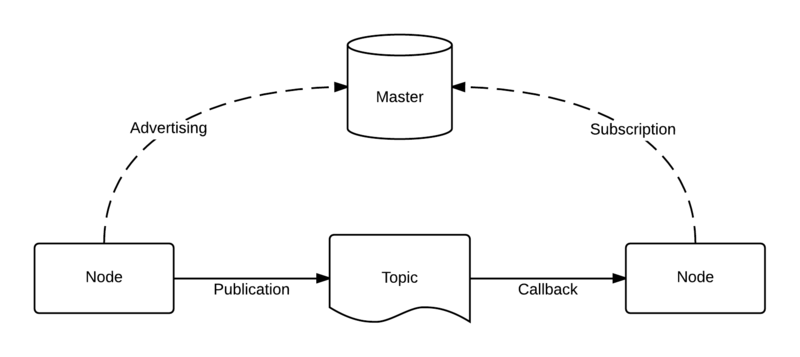
\includegraphics[width=0.8\textwidth]{gfx/master_node_topic}
    \caption[Funzionamento di \emph{master}, \emph{node} e \emph{topic} in \acs{ROS}.]{Funzionamento di \emph{master}, \emph{node} e \emph{topic} in \acs{ROS}.}
    \label{fig:master_node_topic}
\end{figure}

\subsection{Services}
I \emph{services} rappresentano il mezzo di comunicazione sincrono secondo una semantica di tipo request/reply (richiesta/risposta), implementando in \acs{ROS} una funzionalità di tipo \ac{RPC}. Pertanto, si definiscono nella rete nodi provider, che forniscono servizi, e nodi client, che usufruiscono di tali servizi.\\

Esistono funzioni per verificare la presenza di un service provider nella rete. Nel dettaglio, il nodo client invia dei dati che prendono il nome di request a un nodo server, aspettando la risposta di quest’ultimo. Il nodo server, una volta ricevuta, processa la request del client e gli riscontra dei dati in risposta (response).

\subsection{tf}
Quando si eseguono compiti con un robot, è fondamentale che il robot sia consapevole di dove si trova e di dove si trova il resto del mondo rispetto a se stesso. La libreria \emph{tf} \cite{tf} è stata progettata per fornire un modo standard per tenere traccia dei riferimenti di coordinate e trasformare i dati all'interno di un intero sistema in modo tale che gli utenti dei singoli componenti possano essere sicuri che i dati si trovino nel frame di coordinate desiderato, senza richiedere la conoscenza di tutti i riferimenti di coordinate nel sistema. Man mano che i sistemi robotici diventano sempre più complicati, essere in grado di concentrarsi con precisione sul task frame, cioè un frame di coordinate che può essere collegato a diversi oggetti che devono essere manipolati, e sui frame di coordinate rilevanti diventa fondamentale. La maggior parte dei sistemi robotici fonde i dati di molti sensori diversi con frame di coordinate differenti.\\

La libreria \emph{tf} è stata sviluppata come pacchetto \acs{ROS} per fornire questa capacità ed è composta da due moduli standard: un broadcaster (emittente) e un listener (ascoltatore). La prima parte si occupa della diffusione delle informazioni di trasformazione all'intero sistema. La seconda parte riceve le informazioni di trasformazione e le archivia per un uso successivo. Quindi è in grado di rispondere a domande sulla trasformazione risultante tra diversi frame di coordinate.\\

Le trasformazioni e i frame di coordinate possono essere espressi come un grafo con le trasformazioni come archi e i frame di coordinate come vertici. In questa rappresentazione la trasformata netta è semplicemente il prodotto degli archi che collegano due nodi qualsiasi. Il grafo può esistere con uno o più sottografi disconnessi e la trasformazione può essere calcolata tra nodi all'interno dei sottografi (intesi come componente connessa), ma non tra sottografi disconnessi. Tuttavia, in un grafo arbitrario, due nodi possono avere più cammini tra di loro, risultando in due o più potenziali trasformazioni nette che rendono ambiguo il risultato della query. Per evitare questo il grafo deve essere aciclico, in modo che ogni sottografo connesso è un albero. Limitare il grafo a un albero consente una rapida ricerca della connettività. Questo diventa importante con l'aumentare della complessità del grafo. Una struttura ad albero ha anche il vantaggio di consentire modifiche dinamiche alla struttura senza utilizzare informazioni aggiuntive rispetto agli archi del grafo diretto.\\

Il modulo broadcaster è stato progettato in modo molto semplice. Trasmette messaggi ogni volta che si verifica un aggiornamento su una trasformazione specifica.\\

Il modulo listener raccoglie i valori in un elenco ordinato e, quando interrogato, può interpolare tra i due valori più vicini. La frequenza di trasmissione delle trasformate da parte dell'emittente deve essere selezionata sufficientemente alta da consentire la \ac{SLERP} \cite{SLERP}.\\

Per calcolare le trasformazioni tra due nodi qualsiasi, viene calcolato il cosiddetto spanning set. Per calcolare lo spanning set tra un frame di origine e quello di destinazione, il modulo listener risale l'albero (attraverso la relazione di genitore) finché non viene trovato un nodo genitore comune che forma uno spanning set. Se non viene trovato alcun genitore comune, la ricerca fallisce e restituirà un errore. Se la ricerca ha esito positivo, il listener calcolerà la trasformazione netta degli archi dal frame di origine al frame di destinazione lungo il cammino percorso.

\subsection{RViz}
\ac{RViz} è uno strumento di visualizzazione 3D di \acs{ROS}. Consente di visualizzare il robot, il suo orientamento, i sistemi di riferimento, le matrici di covarianza e molto altro. Nell'ambito della tesi è risultato molto utile nelle simulazioni di volo per visualizzare in tempo reale la posizione del drone rispetto al sistema di riferimento a terra.

\begin{figure}[H]
	\begin{center}
	
	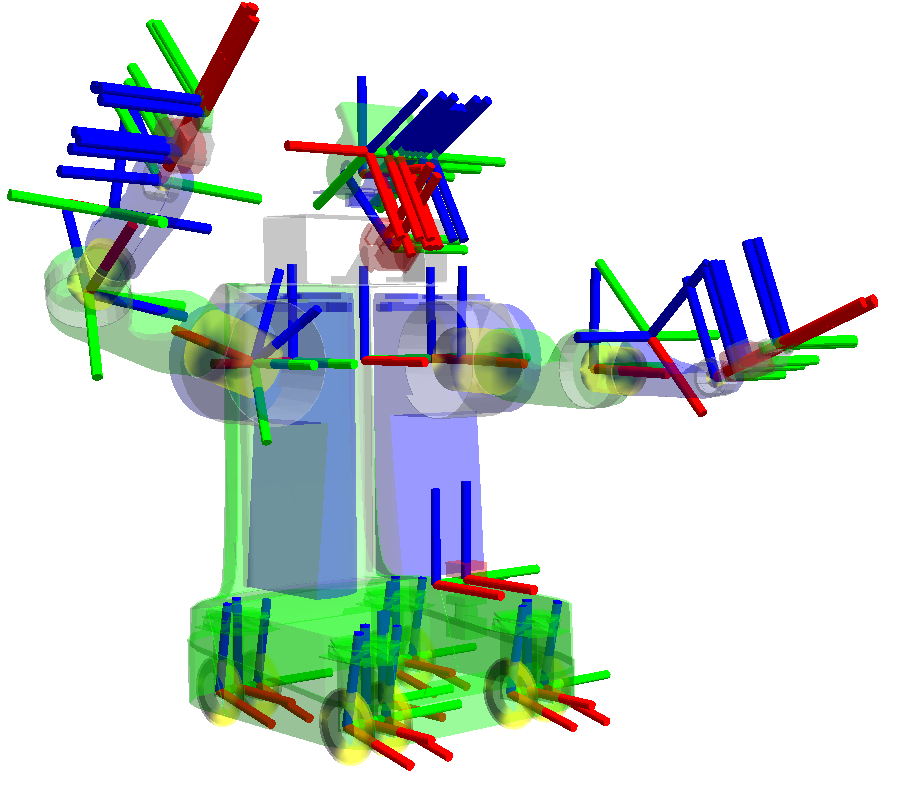
\includegraphics[width=0.55\textwidth]{gfx/tfROS}
    \caption[Task frames nel robot PR2 di Willow Garage.]{Task frames nel robot PR2 di Willow Garage, visualizzate in \acs{RViz}. I cilindri RGB rappresentano gli assi X, Y e Z dei riquadri di coordinate.}
    \label{fig:tf_ROS}
    
    \vspace{30mm}

	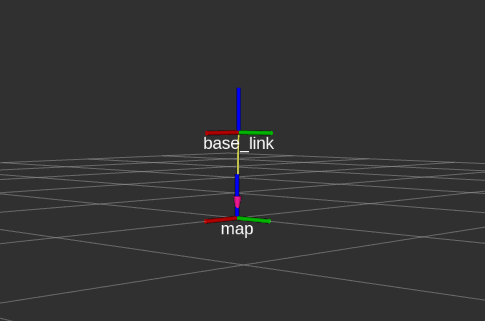
\includegraphics[width=0.7\textwidth]{gfx/ROS/rqt_rviz}
	\caption[Task frames del quadrirotore simulato, in \acs{RViz}.]{Task frames del quadrirotore simulato, visualizzate in \acs{RViz}. Il riferimento del sistema a terra è indicato con \emph{map}, quello solidale al quadrirotore con \emph{base\_link}.}
	\label{fig:droneRviz}
		
	\end{center}
\end{figure}

% ------------------------------ ARCHITETTURA SIM ------------------------------

\section{Architettura Simulazione Quadrirotore}
In questa sezione si entra nel dettaglio dell'architettura di simulazione utilizzata in \acs{ROS}, partendo dalla scelta del sistema operativo. È stato utilizzato il sistema operativo Linux Ubuntu versione 20.04 (Focal Fossa) in quanto compatibile e consigliato per la versione \acs{ROS} adottata (Noetic Ninjemys, rilasciata a Maggio 2020).

\subsection{Gazebo}
Gazebo è un simulatore 3D. Consente di creare uno scenario tridimensionale sul computer con robot, ostacoli e altri oggetti utili alla simulazione del robot in questione.\\

In questo lavoro di tesi, si è fatto uso della repository \emph{iq\_sim} di Intelligent Quads, disponibile su GitHub \cite{iqSIM}. Questa repository contiene mondi gazebo per vari scenari e configurazioni di droni. Inoltre, è specificamente progettata per funzionare con il sistema di controllo ArduPilot e utilizza il plug-in gazebo ArduPilot per consentire al software di controllo ArduPilot di interfacciarsi e controllare il drone in gazebo.

\begin{figure}[H]
	\centering
	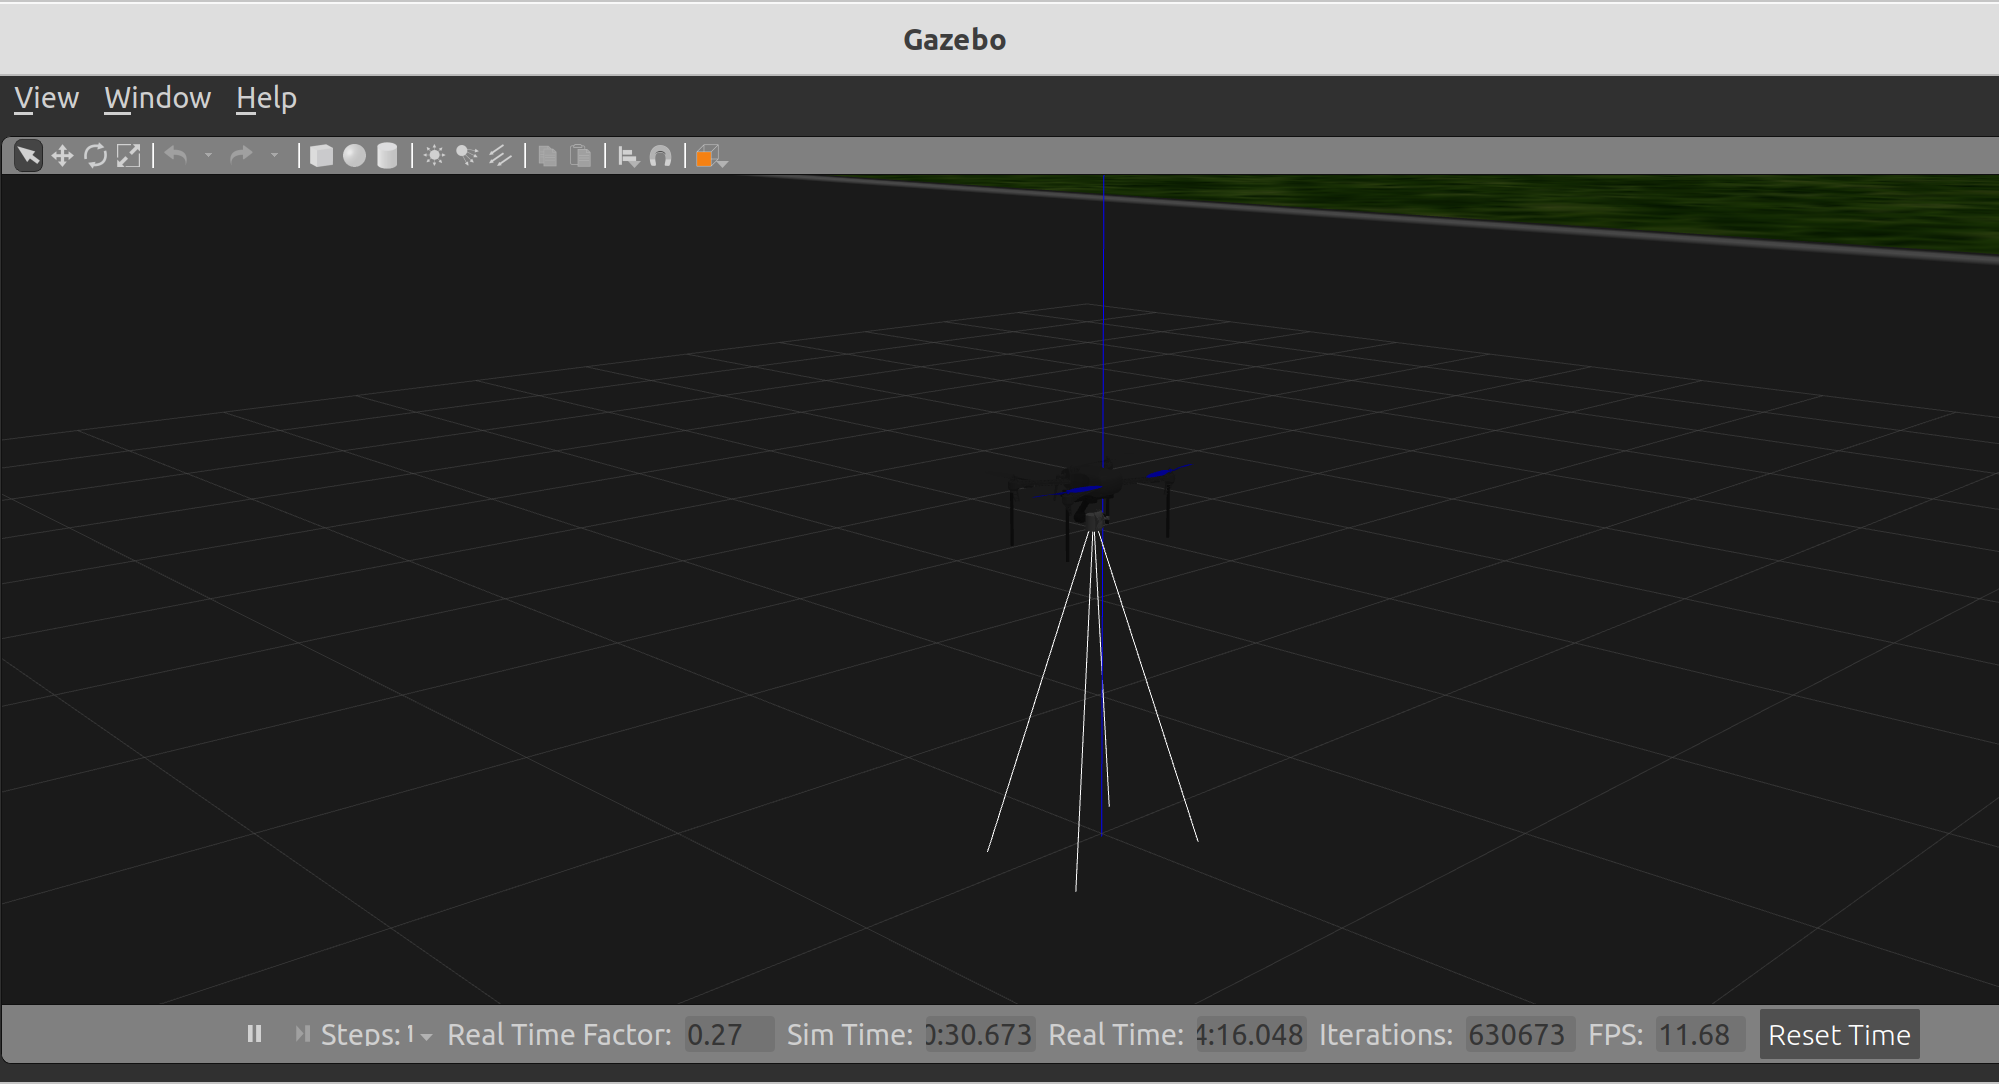
\includegraphics[width=0.7\textwidth]{gfx/ROS/gazebo_new}
	\caption[Quadrirotore nel mondo simulato.]{Quadrirotore nel mondo simulato \emph{runway.world} (pista di decollo) di Intelligent Quads, in Gazebo.}
	\label{fig:gazebo}
\end{figure}

Dopo aver clonato la repository sul computer utilizzato, per lanciare gazebo con il mondo desiderato basta eseguire da terminale il seguente comando.\\

\begin{lstlisting}[language=bash, numbers=none]
  roslaunch iq_sim runway.launch
\end{lstlisting}

\subsection{ArduCopter}
Gli aeromobili a pilotaggio remoto (\acs{UAV}) sono sistemi che richiedono una rapida risposta al variare dei dati forniti dai sensori a bordo, per cui risulta fondamentale per il controllo del volo un software di autopilotaggio. Esistono diverse soluzioni, ma per questa tesi è stato considerato il software ArduCopter, cioè la versione per \acs{UAV} del più generale software ArduPilot.\\

\ac{SITL} \cite{sitl} è un simulatore che consente di eseguire ArduCopter sul computer, senza l'utilizzo di alcun hardware. Per lanciare ArduCopter si esegue il seguente comando da terminale, assicurandosi di essere nella directory corretta di ArduPilot. Le Figure \ref{fig:arduCopter} e \ref{fig:consArduCopter} mostrano le interfacce grafiche contenenti tutte le informazioni sullo stato del velivolo e altri parametri.\\

\begin{lstlisting}[language=bash, numbers=none]
  ./sim_vehicle.py -v ArduCopter -f gazebo-iris --console --mavproxy-args="--streamrate=100"
\end{lstlisting}

\begin{figure}[H]
	\centering
	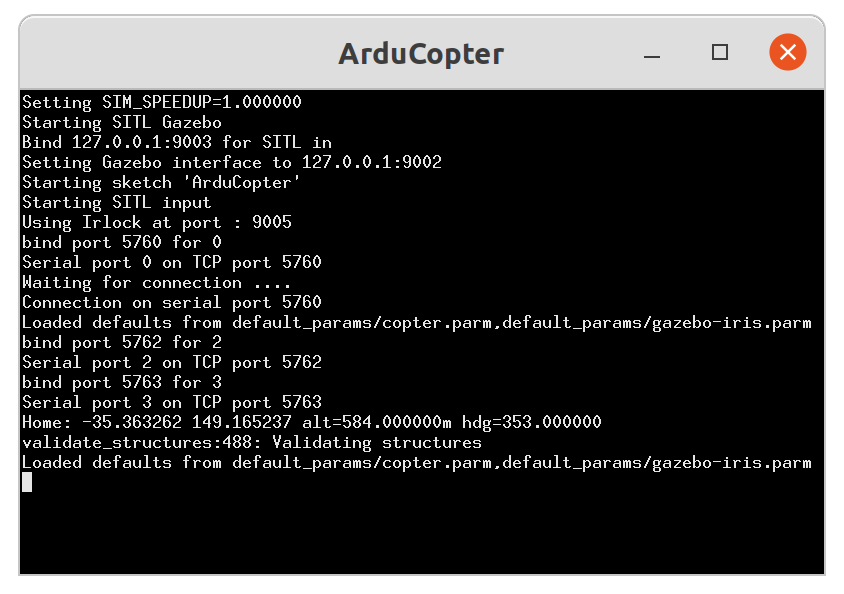
\includegraphics[width=0.55\textwidth]{gfx/ROS/ArduCopter}
	\caption[Interfaccia grafica ArduCopter.]{Interfaccia grafica ArduCopter.}
	\label{fig:arduCopter}
\end{figure}

\begin{figure}[H]
	\centering
	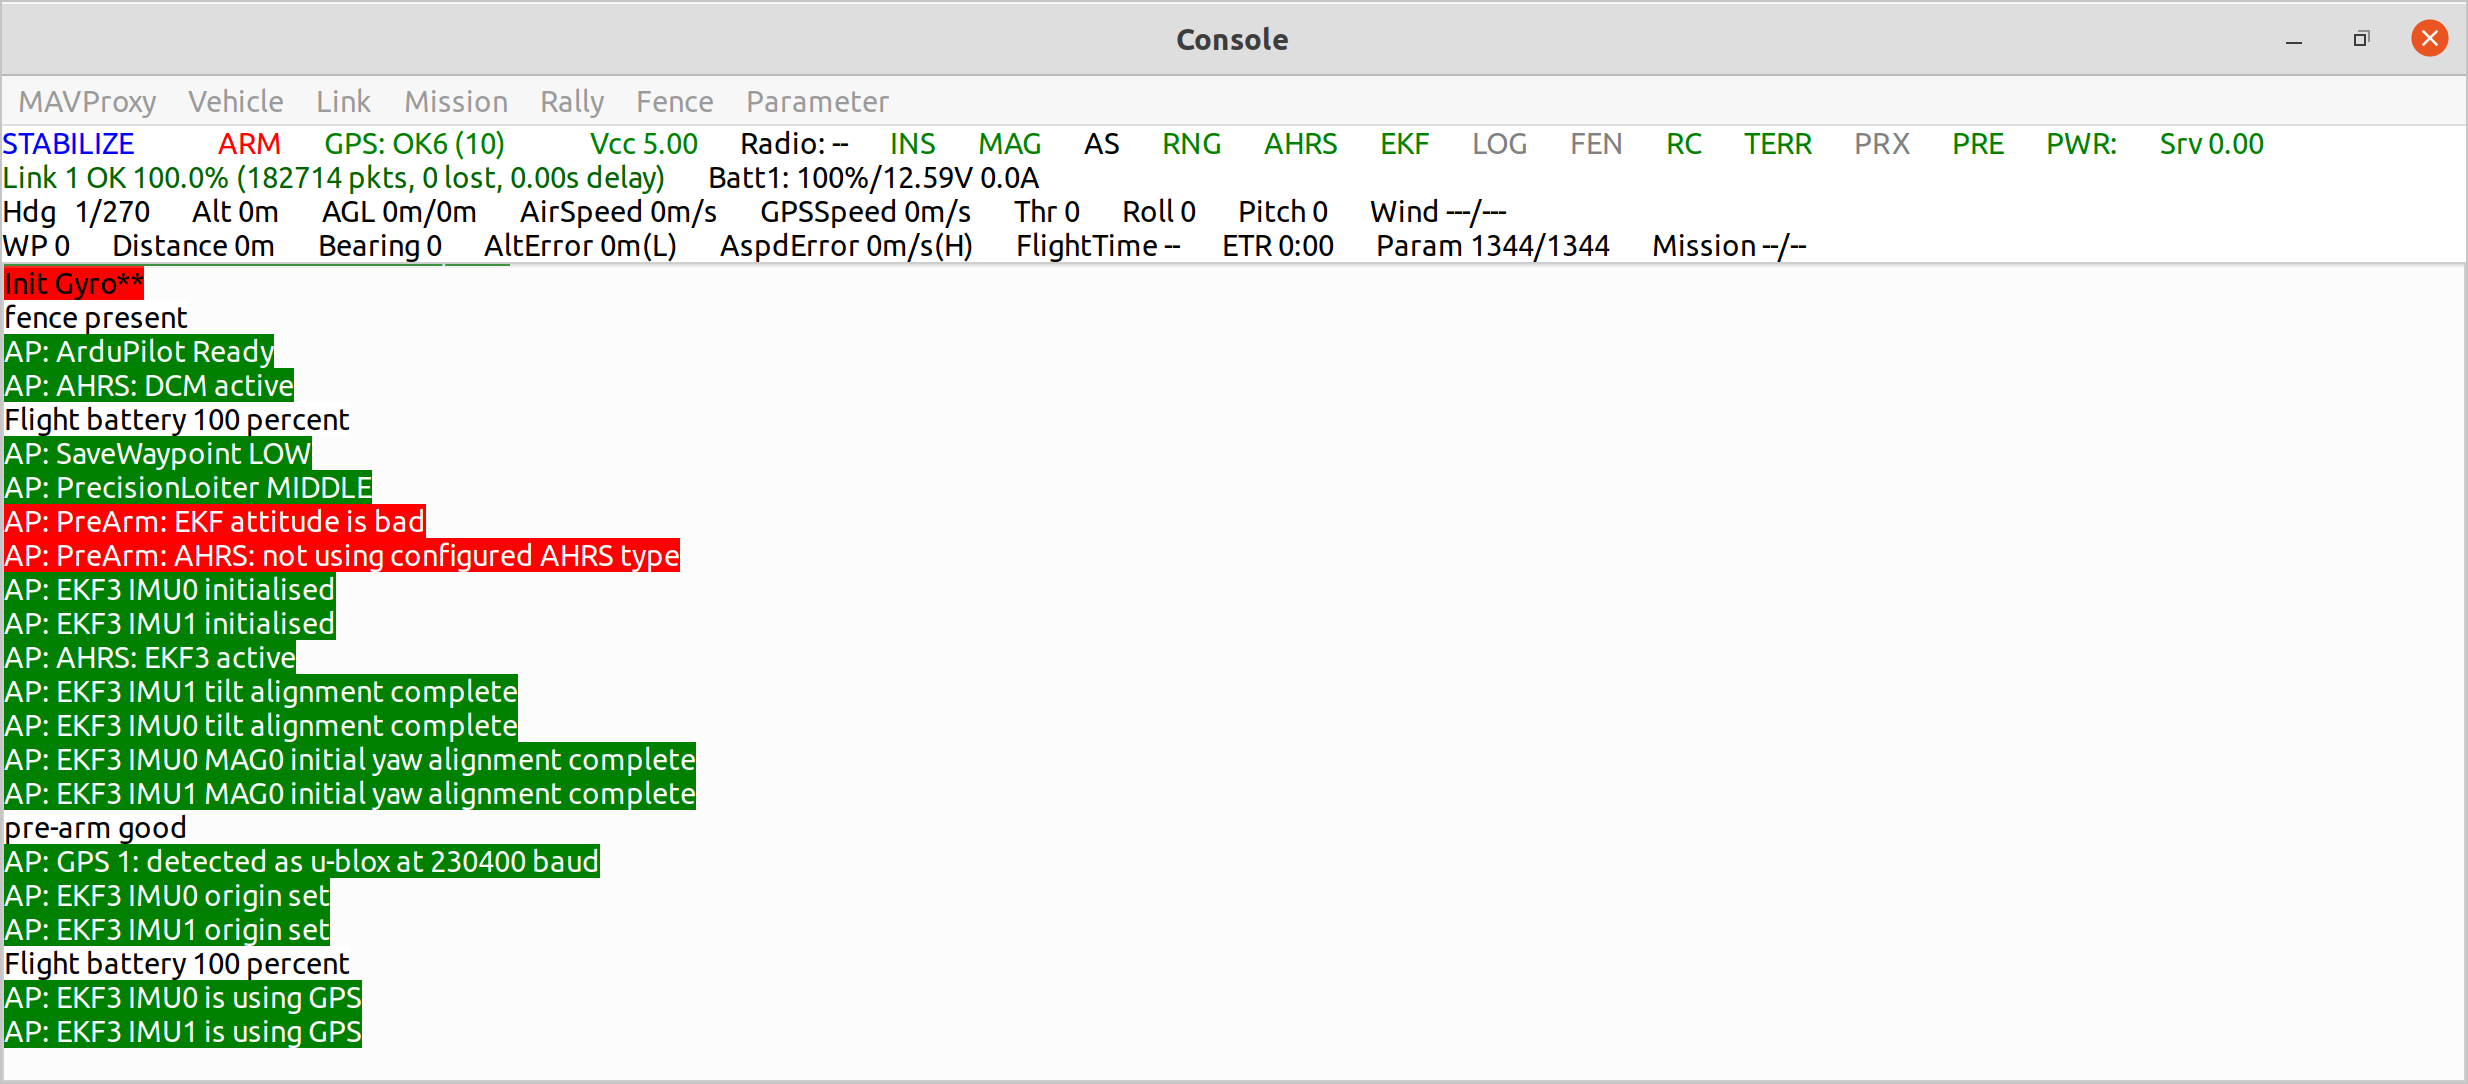
\includegraphics[width=1\textwidth]{gfx/ROS/SITL}
	\caption[Interfaccia grafica console ArduCopter.]{Interfaccia grafica console ArduCopter.}
	\label{fig:consArduCopter}
\end{figure}

\subsection{MAVLink e MAVROS}
MAVLink (Micro Air Vehicle Link) è un protocollo di comunicazione per \acs{UAV} di piccole dimensioni. I pacchetti utilizzati nella comunicazione MAVLink sono strutture in linguaggio C, trasmesse molto efficientemente attraverso dei canali di comunicazione seriale. I punti a suo favore sono sicuramente la velocità di comunicazione, la facilità con cui si possono realizzare nuovi messaggi e il fatto di essere open source. Per quanto riguarda la possibilità di creare nuovi messaggi, MAVLINK permette la definizione mediante file XML (chiamati dialetti), i quali vengono convertiti in codice sorgente in diversi linguaggi in base alle esigenze.\\

MAVROS \cite{mavros} è l'estensione di MAVLink in \acs{ROS}. Tra le tante caratteristiche di MAVROS vale la pena menzionare il fatto che è in grado di convertire i riferimenti di tipo \acs{NED} in riferimenti di tipo \acs{ENU} e viceversa, in modo da essere conforme allo standard adottato in \acs{ROS}.\\

Per completare la configurazione del sistema di simulazione si lancia il file \emph{apm.launch} con il seguente comando da terminale.\\

\begin{lstlisting}[language=bash, numbers=none]
  roslaunch mavros apm.launch
\end{lstlisting}

Questo si occupa di stabilire una connessione tra l'istanza \acs{ROS} in questione e il simulatore configurato precedentemente (Gazebo e ArduCopter). Una delle operazioni più rilevanti, svolta da questo eseguibile, è quella di inviare dati relativi ai \emph{tf} (task frames) coinvolti. In particolare, invia con una certa frequenza di trasmissione dati sui \emph{tf} in modo da mantenerli aggiornati in tempo reale. I \emph{tf} possono essere visualizzati non solo in \acs{RViz}, come mostra la Figura \ref{fig:droneRviz}, ma anche nell'albero dei \emph{tf} (tf\_tree), come mostra la Figura \ref{fig:tf_tree}.

\begin{figure}[H]
	\centering
	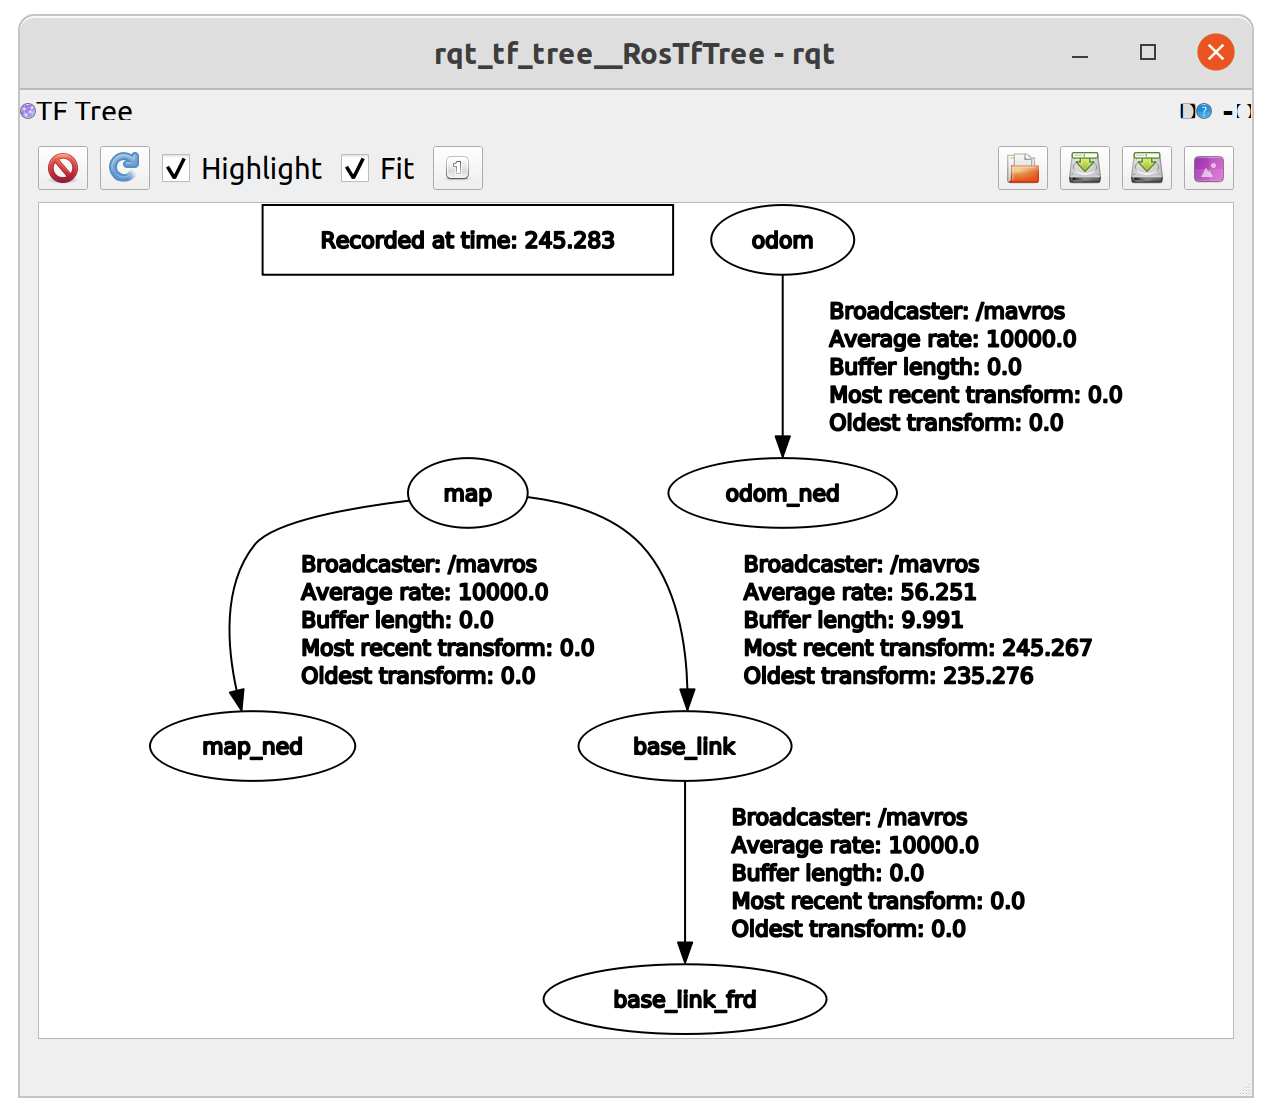
\includegraphics[width=0.75\textwidth]{gfx/ROS/rqt_tf_tree}
	\caption[Task frames del quadrirotore simulato, nel tf\_tree.]{Task frames del quadrirotore simulato, visualizzate nel tf\_tree. Il riferimento del sistema a terra è indicato con \emph{map}, quello solidale al quadrirotore con \emph{base\_link}.}
	\label{fig:tf_tree}
\end{figure}
